\section{Model}
\label{sec:model}

Given input bandwidths $IB_i$ with weights $W_i$ for all clients, we seek to allocate bandwidths $AB_i$ for each
client such that:  

{\bf 1. Congestion Freedom:}  The sum of the allocated bandwidths does not
exceed the bandwidth $B$ of the outbound link. 

{\bf 2. Strong Fair Allocation: } $B$ is divided among active clients in proportion
to their weights $W_i$.

\begin{figure}[t]
\center
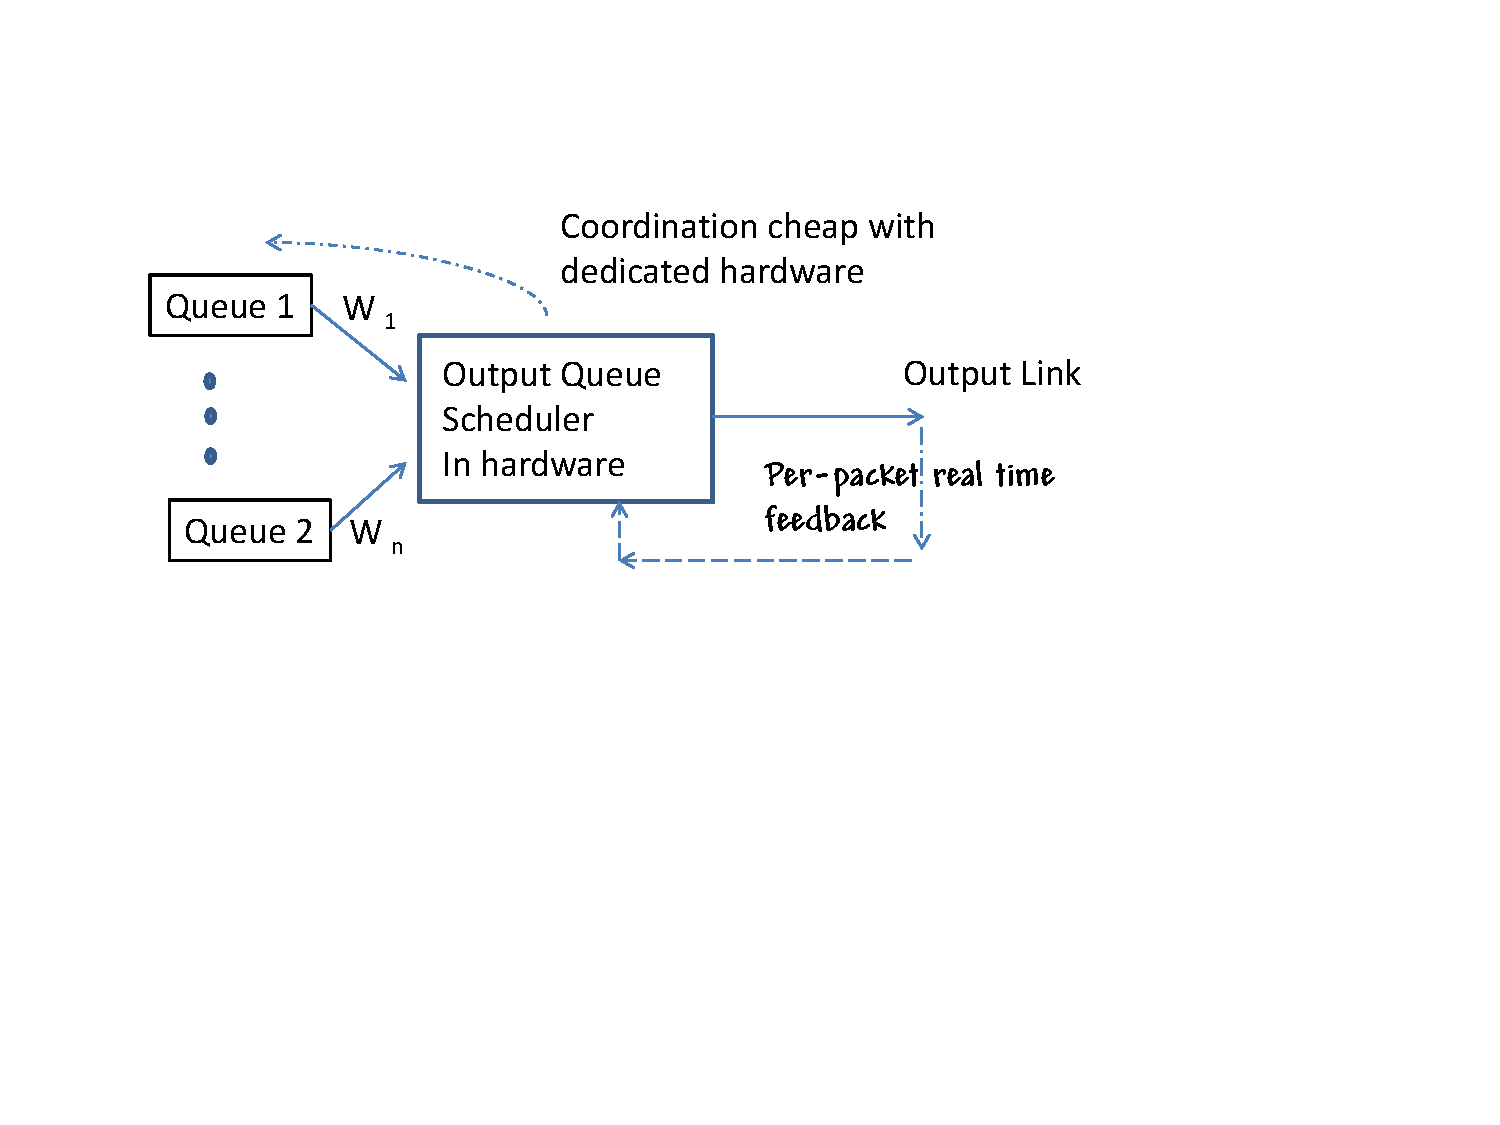
\includegraphics[width=\columnwidth,trim=6mm 90mm 20mm 10mm]{figures/standardqosmodel}
\caption{Standard Fair queuing model}
\label{fig:qosmodel}
\vspace{-2mm}
\end{figure}

Classical fair queuing model including Deficit Round Robin, Start-time Fair Queuing, and Worst Case Weighted Fair
Queuing~\cite{drr, stfq,w2fq, qfq} make two implicit
assumptions. First, after packet transmission the link
alerts the hardware scheduler who chooses the next packet to transmit. Second,
the scheduler is able to keep up with link speed.
Both assumptions are reasonable for hardware routers and switches.

However, in our model  (Figure~\ref{fig:vmqosmodel}) unlike
in Figure~\ref{fig:qosmodel} the feedback
loop between link and scheduler has now become batched.
Since modern NICs use mechanisms like Large Send Offload (LSO) to minimize overhead,
they can only generate one send-complete notification for a group of
packets.  Without per-packet feedback, a DRR software implementation will receive
transmit completion notifications in bursts.   Besides causing transmit jitter, 
the bursts can be far apart with respect to packet arrivals, causing packets to be
dropped. Second, even if the NIC could invoke the scheduler on a per-packet
basis, the cost of running the scheduler after every packet departure will be
prohibitive. It typically takes at least one full core to saturate a 40Gbps link.
 
\begin{figure}
\centering
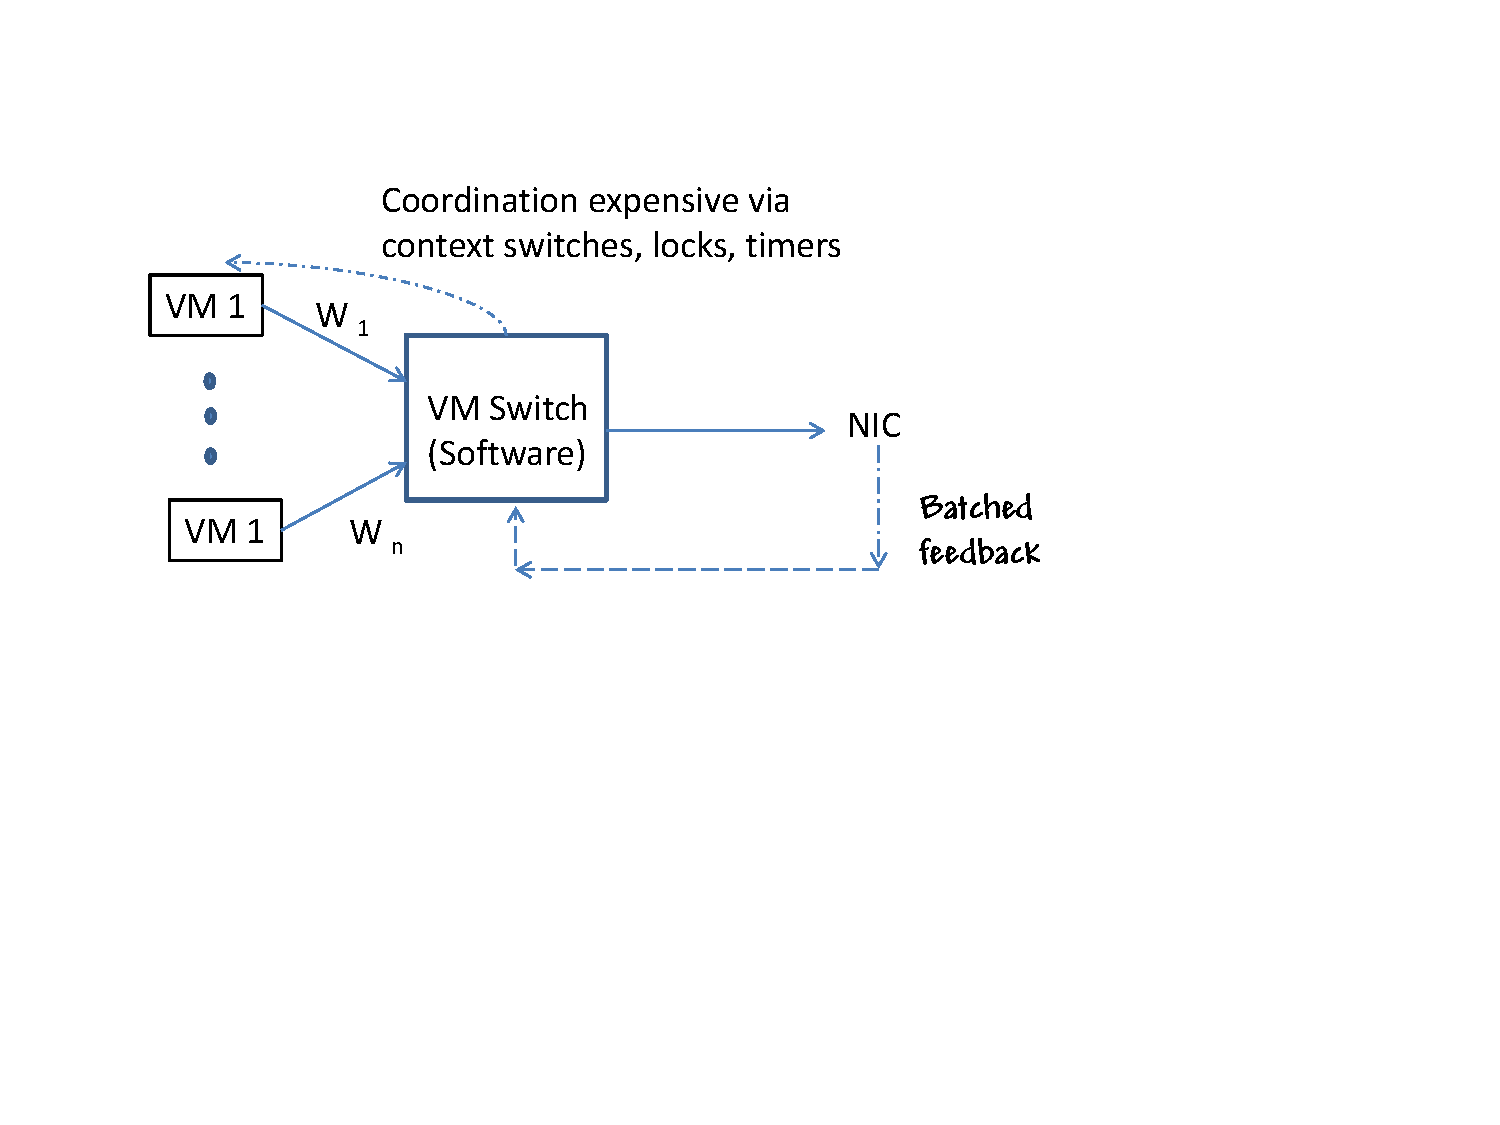
\includegraphics[width=\columnwidth, trim=6mm 90mm 20mm 10mm]{figures/vmqosmodel}
\caption{Model for VM Fair Queuing}
\label{fig:vmqosmodel}
\vspace{-3mm}
\end{figure}

Our model imposes additional constraints.
The software entity that schedules packets from the queues must
ensure that packets are en-queued to the NIC's transmit buffer in the same order
that they are de-queued from VSwitch queues.  

There are two options to achieve this. First, the software could use a handle to
the NIC's transmit buffer.  This requires strong coordination between the
software module and the NIC's driver.  This is not feasible for a software implementation on top of a
hardware abstraction layer (e.g. NDIS in Windows).
 in a general-purpose OS that must work across many NIC vendors

A second alternative is to make the software entity single-threaded so
that each packet is processed sequentially through the entire software stack
from VSwitch to NIC using a single processor. This is not scalable at
multi-gigabit speeds.  Additionally, having to process packets on a single thread
forces packets that were processed on different processors to be then processed
on a different single processor, leading to cache misses which increase latency.

A way out of these difficulties is to divide the scheduler into two enties as
shown in Figure~\ref{fig:macroscheduler}.   The macroscheduler runs only every
$T$ seconds and hence can run on a single thread.   The microschedulers, by
contrast, run on every packet based on tokens allocated by the microscheduler.   

\begin{figure}
\centering
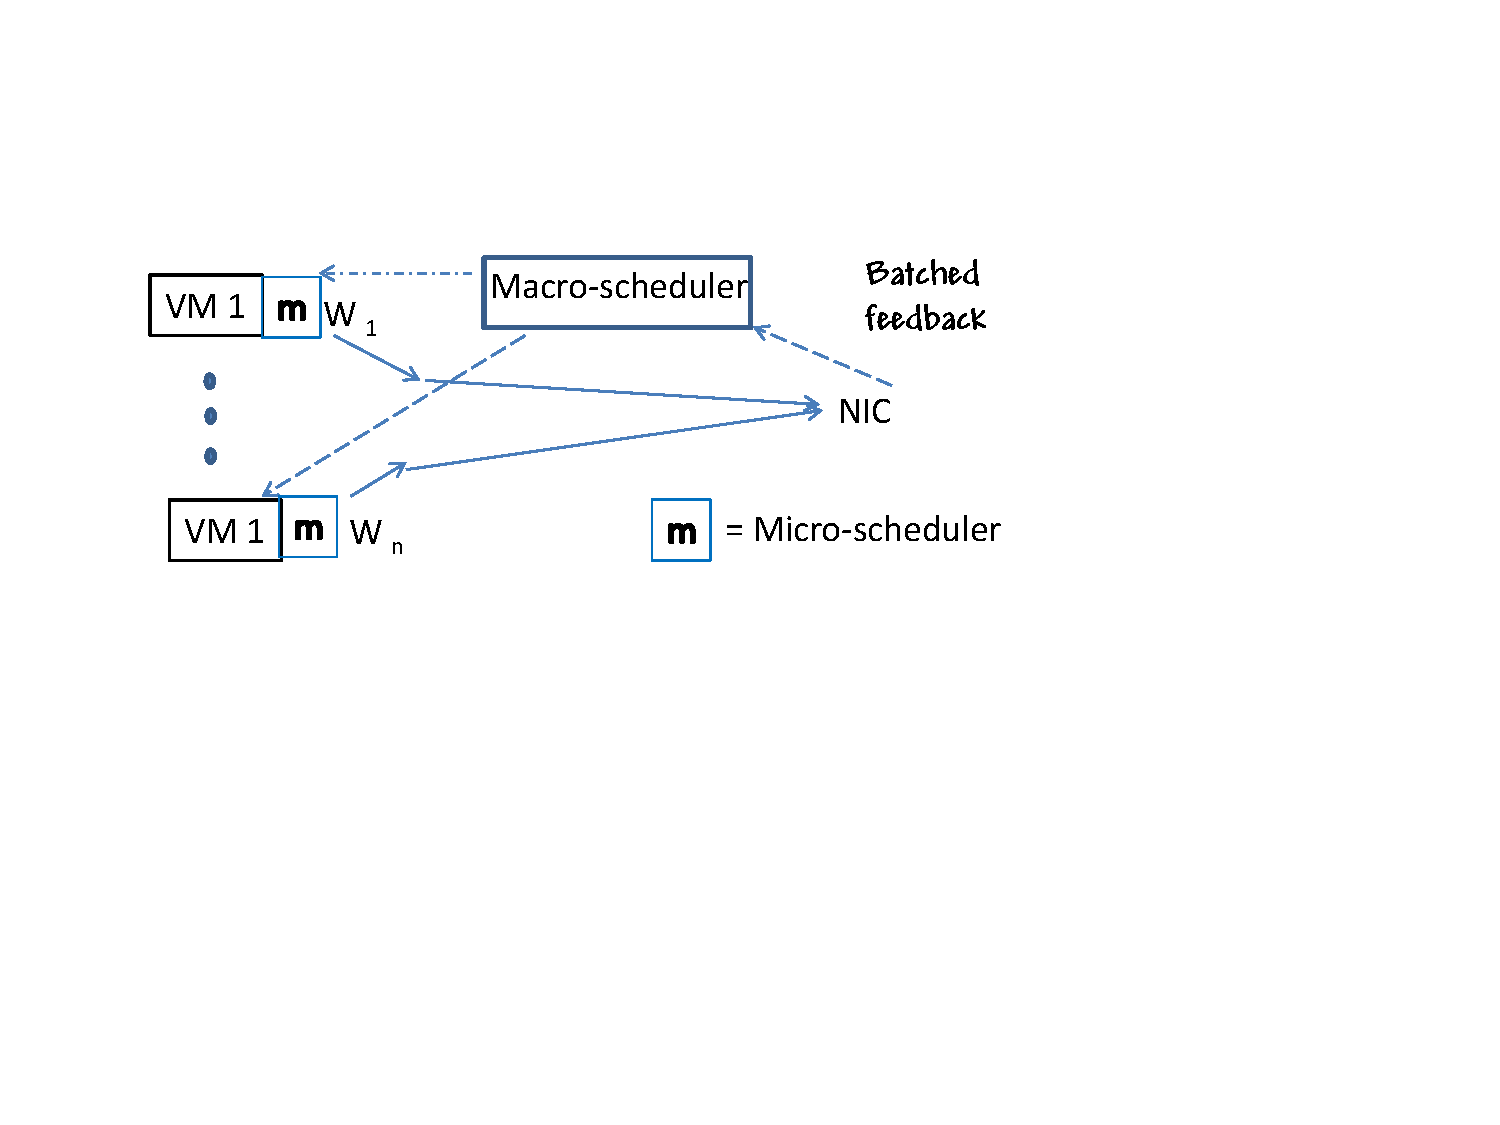
\includegraphics[width=\columnwidth, trim=6mm 90mm 20mm 10mm]{figures/macroschedule}
\caption{Macroscheduler/Microscheduler model}
\label{fig:macroscheduler}
\vspace{-3mm}
\end{figure}

While this model reduces overhead it has obvious drawbacks because allocations
can only occur in units of $T$ seconds.   Thus we have two measures $T_{inc}$
which defines the worst case time for a VM to increase to its guaranteed
bandwidth, and $T_{dec}$ which is the worst case time after a VM decreses below
its allocation till the unused bandwidth is distributed to all active VMs. 
